Ce chapitre présente le bloc qui permet au robot d'exploiter les moteurs et les encodeurs afin de se déplacer. Pour cela, ceux-ci doivent être configurés avant d'être utilisés respectivement comme actionneurs et capteurs dans une boucle fermée de régulation, afin d'obtenir une bonne précision et une résistance aux perturbations. Dans la section suivante, les moteurs et encodeurs ainsi que leur configuration sont brièvement présentés; la régulation sera ensuite couverte.\footnote{Ce chapitre couvre les fichiers \ilcode{wheels.*} et \ilcode{regul.*} du projet \ilcode{propulsion.X}}

\section{Moteurs et encodeurs}
\subsection{Commande en PWM des moteurs}
Les moteurs sont commandé en PWM. Comme le montre la figure \ref{fig:SignalServo}, les paramètres importants à ce bloc sont les suivants:
\begin{itemize}
  \item $\SI{3}{\milli\second} \leq T \leq \SI{20}{\milli\second}$
  \item $ \SI{1}{\milli\second} \leq T_{on} \leq \SI{2}{\milli\second}$
  \item $V_{mot}$ croît linéairement de $-V_{alim}$ à $+V_{alim}$ avec $T_{on}$
  \item $v_{max} \simeq \SI{60}{\centi\meter\per\second}$, $a_{max} \simeq \SI{2}{\meter\per\second\squared}$
  \item Point de fonctionnement suggéré: $v_0 = \SI{40}{\centi\meter\per\second}$, accélération limitée à \SI{50}{\centi\meter\per\second\squared}
\end{itemize}
\begin{figure}[htbp]
\centering
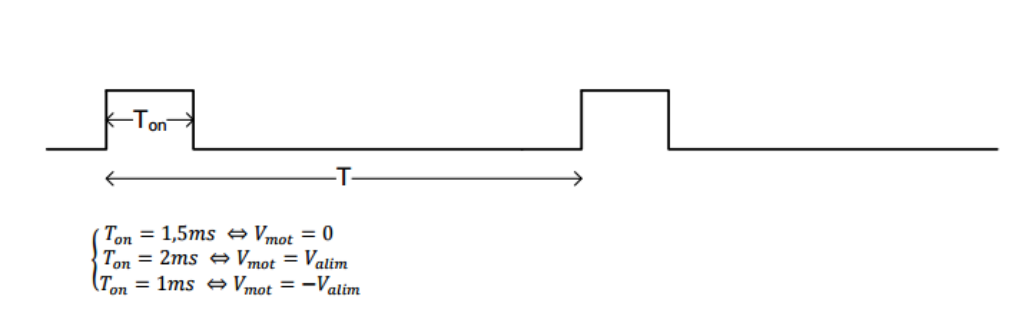
\includegraphics[width=\textwidth]{pwm.png}
\caption{\label{fig:SignalServo}Signal de commande des servomoteurs. [Source: \'Etude du déplacement du robot]}
\end{figure}

Le module output compare du microcontrôleur propulsion suffit à générer cette commande assez simple des moteurs; il sera donc utilisé pour les contrôler. La configuration est opérée par la fonction \ilcode{configPWM()}, qui initialise les paramètres suivants:
\begin{itemize}
  \item Output mapping des ports des output compare sur les pattes physiquement reliées aux moteurs
  \item Choix du mode de PWM: impulsion haute commençant au début de la période et de longueur variable, fixée par \ilcode{OCXRS}
  \item Choix du timer 2 comme valeur de comparaison
  \item Choix de $T_2 = \SI{10}{\milli\second}$, et démarrage du timer 2
\end{itemize}
Une fois $T_2$ fixé, il est plus facile de parler en terme de rapport cyclique ($D$) qu'en longueur arbitraire. Puisque $T_2 = \SI{10}{\milli\second}$, on a directement:
\begin{align*}
  D = 0.1 &\Rightarrow V_{mot} = -V_{alim}\\
  D = 0.15 &\Rightarrow V_{mot} = 0\\
  D = 0.2 &\Rightarrow V_{mot} = +V_{alim}\\
\end{align*}
La commande en tension des moteurs est donc finalement imposée par une simple instruction du type \ilcode{OCXRS = $D$*PR2}. $D$ sera donc la sortie du régulateur.

\subsection{Encodeurs en quadrature}
La rotation de chaque roue est mesurée par un encodeur en quadrature dont les paramètres importants sont les suivants:
\begin{itemize}
  \item 90 impulsions montantes par tour de roue;
  \item Pas de détection d'un tour de roue complet;
\end{itemize}
La sortie des encodeurs est traitée par le module QEI du microcontrôleur propulsion. Le module est configuré comme suit par la fonction \ilcode{configQEI()}:
\begin{itemize}
  \item Input mapping des pattes physiquement reliées aux encodeurs sur les ports des QEI;
  \item Choix du mode 4X sans index (pas disponible sur les encodeurs utilisé): 360 impulsions par tour de roue;
  \item Choix du maximum des compteurs à 360, et activation de l'interruption lorsqu'un compteur overflow, ce qui permet de reproduire le mécanisme d'index et de compter les tours de roues, afin de n'avoir virtuellement aucune limite sur les distances à mesurer (en cas d'utilisation prolongée, par exemple);
\end{itemize}
Les routines d'overflow sont extrêmement simples: \ilcode{xSpins} est simplement incrémentée ou décrémentée en fonction de \ilcode{QEIxCON.UDPN}.

L'interface des encodeurs pour la régulation est la fonction \ilcode{readDistances} pour chaque roue, la distance parcourue en centimètres est donnée par:
\[
  \mathtt{d_x} = (\mathtt{xSpins} \cdot \mathtt{MAXxCNT} + \mathtt{POSxCNT})\cdot\mathtt{CM\_PER\_TICK}
\]
\ilcode{readDistances()} sera donc la sortie du capteur de la régulation.



\subsection{Validation des moteurs et encodeurs\label{sec:validMotor}}
L'implémentation de \ilcode{wheels.c} est validée en fixant $D$ à une certaine valeur ($\neq 0.15$) et en vérifiant que le robot se déplace bien et que les mesures de position des roues sont correctes. Les tests sont concluants, les encodeurs sont entièrement satisfaisants, mais les moteurs semblent posséder une zone morte\footnote{Celle-ci se manifeste même lorsque les roues ne sont pas en contact avec le sol, et l'inertie du robot n'est donc pas le seul facteur.} non négligeable qui varie en plus entre les deux roues et avec le temps\footnote{Et probablement la charge de la batterie}. Les moteurs sont aussi généralement dissymétriques, c'est à dire qu'à un même $D$ donné correspondent des vitesses gauche et droite différentes. C'est bien sûr le rôle de la régulation de rejeter le mieux possible ces perturbations, comme nous allons le voir dans la section suivante.

\section{Régulation}
Avant d'aborder le c\oe{}ur du problème, c'est à dire l'implémentation du régulateur, le code qui permet de fermer la boucle et d'utiliser le régulateur est d'abord présenté.
\subsection{Configuration minimale}
Les commandes des moteurs sont mises à jour à intervalles réguliers par la régulation, un timer est donc nécessaire. La configuration de la régulation est opérée par \ilcode{configRegul()}, qui effectue les actions suivantes:
\begin{itemize}
  \item Choix de la période du timer 1 ($f_{regul} = f_{OC} = \SI{100}{\hertz}$) et démarrage de celui-ci
  \item Initialisation de certaines variables d'état et des consignes
  \item Activation de l'interruption du timer 1
\end{itemize}

C'est dans la routine d'interruption du timer 1 que toute le boucle fermée se déroule et que le microcontrôleur propulsion passe la plupart de son temps d'exécution. Les actions suivantes sont effectuées durant la routine de régulation:
\begin{itemize}
  \item Lecture des encodeurs à l'aide de \ilcode{readDistances()}
  \item Calcul des $D$ par le régulateur
  \item Mise à jour des commandes par \ilcode{OCxRS = $D_x$*PR2}
  \item Mise à jour des consignes
  \item Détection de l'arrivée du robot à sa position visée
\end{itemize}

Nous pouvons maintenant enfin aborder la conception du régulateur, et la génération de ses consignes.

\subsection{Conception et implémentation du régulateur}
\subsubsection{Choix du schéma de régulation MIMO}
Il est suggéré de mettre en place deux régulateurs proportionnels indépendants agissant sur la position des roues. Deux régulateurs indépendants constituent la solution la plus simple, tandis qu'une régulation de position permet de bénéficier d'un intégrateur et donc d'une erreur statique théoriquement nulle sur la vitesse. Le déplacement en ligne droite serait obtenu en donnant des consignes identiques aux deux roues, et la rotation en donnant des consignes opposées.

Cette régulation est cependant fortement dégradée par les zones mortes variables dont nous avons parlé à la section \ref{sec:validMotor}. Lorsque le robot est muni d'un tel régulateur, ces zones mortes se manifestent par un changement de direction du robot avant de commencer le déplacement en ligne droite. En effet, puisqu'un moteur sort forcément de sa zone morte (bien) avant l'autre, le robot commence par tourner autour de sa roue immobile avant de commencer à avancer. Ceci est l'effet le plus visible, mais on constate aussi que le robot dévie de sa trajectoire. Tout ceci ne peut pas être compensé par la régulation suggérée, qui assure simplement que les deux roues aient parcouru la même distance, mais pas forcément dans le même temps. Il y a plusieurs solutions à ce problème.

La première solution consiste à augmenter le gain de façon à ce que le temps d'établissement soit le plus court possible. En effet, c'est pendant cette durée que les effets de dissymétrie ont lieu (puisqu'après les positions sont par définition calées sur les consignes). Cependant, ceci fait apparaître des oscillations puis des instabilités et est limité par la saturation des moteurs. Même le gain le plus grand possible n'est pas suffisant pour compenser l'effet des dissymétries.

La deuxième solution consiste à essayer de caractériser le mieux possible les zones mortes et les dissymétries entre les deux moteurs, pour par exemple introduire un offset dans les commandes des moteurs et utiliser des gains différents sur les deux régulateurs. Cette alternative est limitée par la précision des mesures et du modèle choisi, et par la dérive des valeurs avec le temps et d'autres facteurs.

La troisième et dernière solution est beaucoup plus fondamentale et constructive: elle consiste à essayer de concevoir un régulateur qui, par design, est supposé être capable de rejeter les dissymétries entre les moteurs. Pour cela le régulateur opère non plus sur les positions séparées des deux roues, mais sur la distance parcourue et la rotation du robot. Le déplacement en ligne droite est obtenu en donnant une consigne non nulle de distance parcourue et une consigne nulle de rotation, et vice-versa pour la rotation, ce qui a l'avantage d'être aussi un peu plus naturel. Les deux régulateurs sont toujours proportionnels, et on conserve la propriété d'intégration qui assure une erreur statique nulle. C'est cette régulation-ci que nous avons finalement choisi.

\subsubsection{Implémentation du régulateur choisi}
Pour calculer la distance totale parcourue, nous utilisons les relations suivantes:
\begin{align*}
  v_l &= \frac{v_{right}+v_{left}}{2}\\
  \omega_z &= \frac{v_{right} - v_{left}}{l_{axis}}
\end{align*}
L'intégration est immédiate, $d_l$ et $\theta_z$ s'expriment simplement à partir des lectures des encodeurs:
\begin{align*}
  d_l(t) = \int_0^tv_l dt &= \frac{d_{right}+d_{left}}{2}\\
  \theta_z(t) = \int_0^t \omega_z dt &= \frac{d_{right} - d_{left}}{l_{axis}}
\end{align*}
Ces expressions sont implémentées par \ilcode{readDistances()}.

L'implémentation du régulateur proportionnel est ensuite extrêmement simple et se trouve dans la fonction \ilcode{setPWMs(float distance)}. Les gains sont trouvés expérimentalement. Ils sont différents selon que le robot est à l'arrêt, en rotation ou en déplacement en ligne droite. En effet, selon le mouvement en cours, un des $k_p$ sert au suivi de consigne, tandis que l'autre sert à la réjection des perturbations, et est donc logiquement plus important\footnote{A l'arrêt, les deux gains servent bien sûr à la réjection de perturbations.}.

\subsubsection{Génération des consignes}
Les consignes de distance parcourue et de rotation sont générées par intégration à partir d'un profil trapézoïdal de vitesse, comme le suggère la figure \ref{fig:vConsigne}, extraite de l'étude du déplacement reçue.
\begin{figure}[htbp]
  \centering
  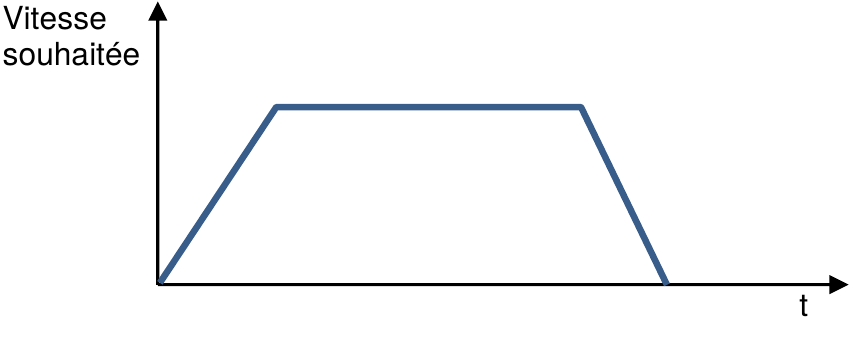
\includegraphics[width = 0.7\textwidth]{vConsigne.png}
  \caption{Profil de vitesse trapézoïdal.[Source: \'Etude du déplacement du robot]\label{fig:vConsigne}}
\end{figure}
La fonction \ilcode{updateConsignes()} génère les consignes. Il s'agit simplement d'une double intégration de l'accélération (angulaire) puis de la vitesse (angulaire), avec en plus une mise à zéro de l'accélération (angulaire) lorsque la vitesse dépasse la vitesse (angulaire) de croisière.

\subsubsection{Détection de l'arrivée}
La fonction \ilcode{checkTerminalCondition()} est responsable de donner une valeur d'accélération (angulaire) opposée à la vitesse (angulaire) lorsque l'objectif est distant de la distance de décélération, et d'ensuite annuler la vitesse (angulaire) et l'accélération (angulaire) lorsque la vitesse (angulaire) change de signe. Le choix de la distance de décélération est plus détaillé dans la section \ref{sec:stateVars}.

\section{Validation du bloc <<déplacement>>}
Chronologiquement, nous avons implémenté les fonctions \ilcode{straight(char distance)} et \ilcode{rotate(char angle, char way)} de \ilcode{decision.c}, présentées dans le chapitre \ref{chap:decision}, immédiatement après la régulation, notamment pour la tester. Il suffit donc d'appeler une de ces fonctions dans le main pour tester la régulation. Dans l'ensemble, celle-ci est satisfaisante, et permet d'effectuer tous les déplacements demandés et l'arrêt immédiat. On remarque cependant que la précision relative sur des courtes distances et sur les rotations\footnote{Celles-ci demandent toujours des courtes distances parcourues par chacune des roues.} n'est pas très bonne. Ceci est dû à la précision limitée des encodeurs\footnote{$\sim\frac{1}{360}$ de tour $ = \SI{0.09}{\centi\meter}$, donne une borne absolue sur la précision, mais celle-ci n'est de loin jamais atteinte.} mais surtout aux moteurs et leurs zones mortes, auquel s'ajoute le fait que la régulation garantit théoriquement une erreur statique nulle sur la vitesse, mais pas sur la position.

Nous disposons maintenant d'un bloc déplacement complet et fonctionnel, nous allons maintenant repartir <<par l'autre côté>> pour aborder la réception des instructions, en commençant donc par la chaîne d'acquisition audio.
